\documentclass[12pt]{article}

\usepackage[utf8]{inputenc}
%\usepackage[T1]{fontenc}

\usepackage{geometry}
\geometry{a4paper}
\usepackage{graphicx}
\usepackage{float}
\usepackage[italian]{babel}

\linespread{1.2}
\setlength{\parindent}{0pt}

\begin{document}

\renewcommand{\labelenumii}{\arabic{enumi}.\arabic{enumii}}
\renewcommand{\labelenumiii}{\arabic{enumi}.\arabic{enumii}.\arabic{enumiii}}
\renewcommand{\labelenumiv}{\arabic{enumi}.\arabic{enumii}.\arabic{enumiii}.\arabic{enumiv}}
%----------------------------------------------------------------------------------------
%	TITOLO
%----------------------------------------------------------------------------------------

\begin{titlepage}

\newcommand{\HRule}{\rule{\linewidth}{0.5mm}}

\center

\textsc{\Large Relazione di progetto di "Smart City e Tecnologie Mobili"}\\[0.5cm]

\HRule \\[0.4cm]
{ \huge \bfseries CityTwin}\\[0.4cm]
\HRule \\[1.5cm]

\vfill

\begin{flushleft}
\emph{Numero del gruppo: 128}\\[1cm]
\emph{Componenti del gruppo: Eddie Barzi, Filippo Vissani}\\[3cm]
\end{flushleft}

\end{titlepage}

%----------------------------------------------------------------------------------------
%	INDICE
%----------------------------------------------------------------------------------------

\tableofcontents

\newpage

%----------------------------------------------------------------------------------------
%	INTRODUZIONE
%----------------------------------------------------------------------------------------

\section{Introduzione}

Il progetto CityTwin si propone di realizzare la simulazione di un sistema di digital twin nel contesto della smart city. In particolare, si vuole realizzare un sistema che sia in grado di catturare e rappresentare in formato digitale il comportamento delle varie entità presenti all'interno della città. Questo può portare ad una serie di benefici, alcuni dei quali vengono elencati di seguito:

\begin{itemize}
    \item Rilevazione di possibili problematiche e intervento tempestivo/automatizzato.
    \item Riduzione del consumo energetico.
    \item Rilevazione della qualità dell'aria e dell'acqua.
    \item Analisi dell'inquinamento acustico.
    \item Ottimizzazione della mobilità urbana.
\end{itemize}

La simulazione sarà composta da due tipologie di nodi: i nodi Mainstay, che rappresentano la struttura portante del sistema, e i nodi Resource, che rappresentano astrazioni di sensori, attuatori o entità più complesse.

I nodi Mainstay si occupano di scambiare informazioni con i nodi Resource, rilevare eventuali malfunzionamenti e salvare in modo persistente le informazioni rilevate dai nodi Resource. I nodi Mainstay devono essere sempre sincronizzati tra loro, in modo da poter garantire la coerenza dei dati.

I nodi Resource, invece, si occupano di rilevare informazioni e comunicarle ai nodi Mainstay nel caso in cui vengono considerati come sensori. Nel caso in cui i nodi Resource rappresentino attuatori, invece, si occupano di ricevere informazioni dai nodi Mainstay e agire di conseguenza.

Per la memorizzazione delle dello stato dei nodi viene disposto un servizio apposito di persistenza dei dati. Tale servizio viene utilizzato sia dai nodi Mainstay che da altri clienti, come ad esempio il pannello di controllo.

L'utente potrà visualizzare lo stato attuale del sistema, lo storico dei dati ed eventuali statistiche, nonché interagire con il sistema tramite GUI, ad esempio per intervenire dopo la rilevazione di un incendio.

Per la realizzazione del progetto verranno utilizzate le seguenti tecnologie:

Akka è un toolkit open source e runtime che semplifica la costruzione di applicazioni concorrenti e distribuite sulla JVM. Questo toolkit supporta diversi modelli di programmazione per la concorrenza, ma enfatizza la concorrenza basata su attori.

I componenti principali del progetto, quali Mainstay e Resource, verranno modellati sulla base del paradigma ad attori e verranno realizzati utilizzando Akka in combinazione con il linguaggio Scala 3.

Per quanto riguarda il servizio di persistenza dei dati, utile per visualizzare le statistiche, verrà utilizzato MongoDB, un database non relazionale orientato ai documenti. Questo database verrà utilizzato per salvare in modo persistente i dati rilevati dai nodi Mainstay.
Il servizio di persistenza verrà realizzato come modulo separato, per questo motivo si sceglie di implementare un layer scritto in JavaScript, che esponga delle API utilizzabili sia dai nodi Mainstay che da altri clienti.

Sulla base dei linguaggi scelti, verranno adottati Simple Build Tool (SBT) per Scala 3 e Node Package Manager (NPM) per JavaScript per la gestione delle dipendenze e la compilazione del codice.

Per semplificare l'avvio del sistema distribuito e garantire la scalabilità verrà utilizzato Docker, un progetto open source che automatizza il deployment di applicazioni all'interno di contenitori software.

\newpage

%----------------------------------------------------------------------------------------
%	STATO DELL'ARTE
%----------------------------------------------------------------------------------------

\section{Stato dell'arte}



\newpage


%----------------------------------------------------------------------------------------
%	ANALISI DEI REQUISITI
%----------------------------------------------------------------------------------------

\section{Analisi dei requisiti}

Di seguito viene riportato l'elenco dettagliato dei requisiti del sistema.

\begin{enumerate}
    \item I nodi Mainstay sono la struttura portante dell'intero sistema:
    \begin{enumerate}
        \item Ricevono informazioni dai nodi Resource che modellano sensori.
        \item Comunicano informazioni ai nodi Resource che modellano attuatori.
        \item Rilevano i malfunzionamenti dei nodi Resource.
        \item Rilevano i malfunzionamenti degli altri nodi Mainstay.
        \item Si occupano di salvare le informazioni contattando il servizio di persistenza.
        \item Non devono conoscere a prescindere le tipologie dei nodi Resource.
        \item Devono disporre di una struttura dati distribuita che permetta di memorizzare le informazioni rilevanti:
        \begin{enumerate}
            \item La struttura dati deve essere sincronizzata tra i nodi Mainstay.
            \item La struttura dati deve mantenere la consistenza dei dati nel tempo.
        \end{enumerate}
    \end{enumerate}
    \item I nodi Resource:
    \begin{enumerate}
        \item Rappresentano astrazioni di:
        \begin{enumerate}
            \item Sensori.
            \item Attuatori.
            \item Entità più complesse, come stazioni di controllo, che possono anche impiegare interfacce grafiche.
        \end{enumerate}
        \item Fanno riferimento ad uno dei nodi Mainstay per ottenere o comunicare informazioni.
        \item Possono essere aggiunti o rimossi in tempo reale.
    \end{enumerate}
    \item Deve essere presente una GUI (distinta da quelle definite al punto 2.1.3) con le seguenti funzionalità:
    \begin{enumerate}
        \item Deve mostrare lo stato attuale dei nodi Mainstay e Resource del sistema.
        \item Deve mostrare la posizione delle risorse nella città.
        \item Deve presentare alcune statistiche interessanti sulla base dei dati rilevati dal servizio di persistenza.
    \end{enumerate}
    \item Deve essere presente un servizio di persistenza dei dati che permetta di salvare in modo persistente:
    \begin{enumerate}
        \item Lo stato dei nodi Mainstay.
        \item Lo stato dei nodi Resource.
    \end{enumerate}
    \item Il malfunzionamento di un nodo non deve compromettere il funzionamento del sistema.
    \item Il sistema deve essere realizzato in moduli separati, in modo da poter essere facilmente estendibile.
    \item Deve poter essere possibile introdurre nuovi moduli senza dover modificare i componenti esistenti.
    \item Vengono previsti i seguenti moduli per i nodi Resource:
    \begin{enumerate}
        \item Sensore per la rilevazione di piogge acide.
        \item Sensore per l'analisi della qualità dell'aria.
        \item Sensore per la rilevazione dell'inquinamento acustico.
        \item Modulo per la rilevazione del livello dell'acqua di un fiume e possibilità di intervento:
        \begin{enumerate}
            \item Sensore per la rilevazione degli allagamenti.
            \item Pannello di controllo per l'intervento in caso di allagamento.
        \end{enumerate}
    \end{enumerate}
\end{enumerate}

\newpage


%----------------------------------------------------------------------------------------
%	PROGETTAZIONE
%----------------------------------------------------------------------------------------

\section{Progettazione}

\begin{figure}[h]
\caption{Diagramma dei componenti del sistema e delle loro dipendenze.}
    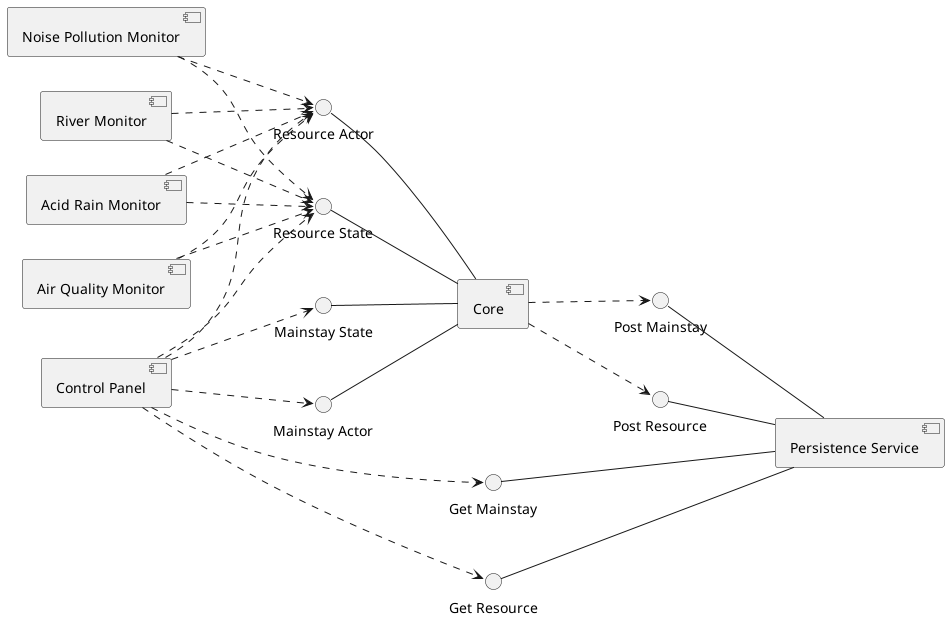
\includegraphics[width=\textwidth]{../assets/images/core-component-diagram.png}
\end{figure}

\begin{figure}[h]
    \caption{Diagramma delle classi del modulo \textit{Core}.}
    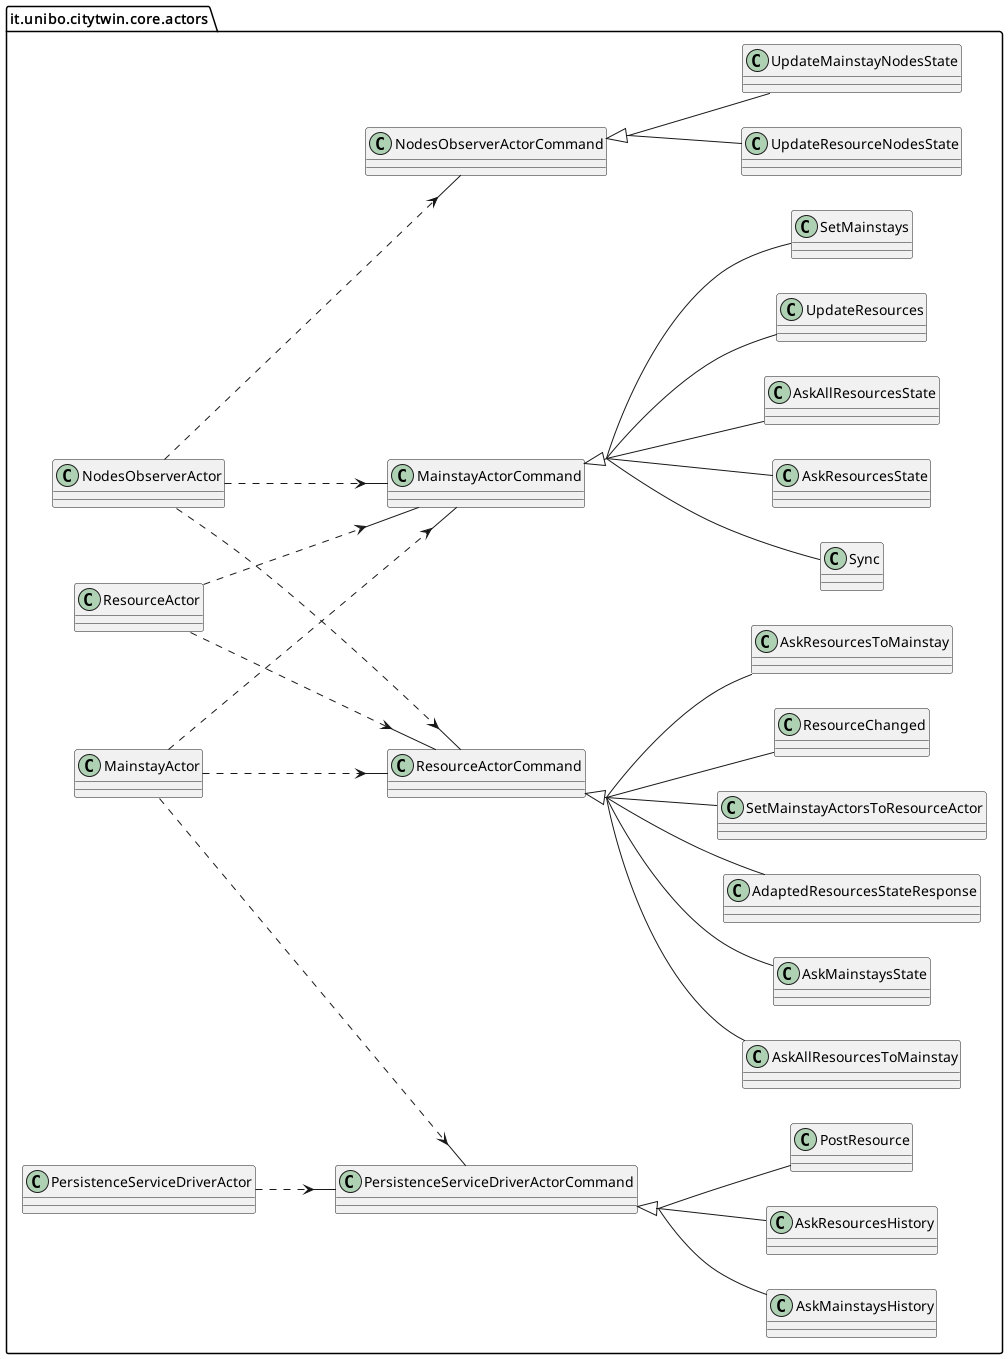
\includegraphics[width=\textwidth]{../assets/images/core-class-diagram.png}
\end{figure}

\begin{figure}[h]
    \caption{Diagramma dei componenti in esecuzione e dei protocolli di rete utilizzati.}
    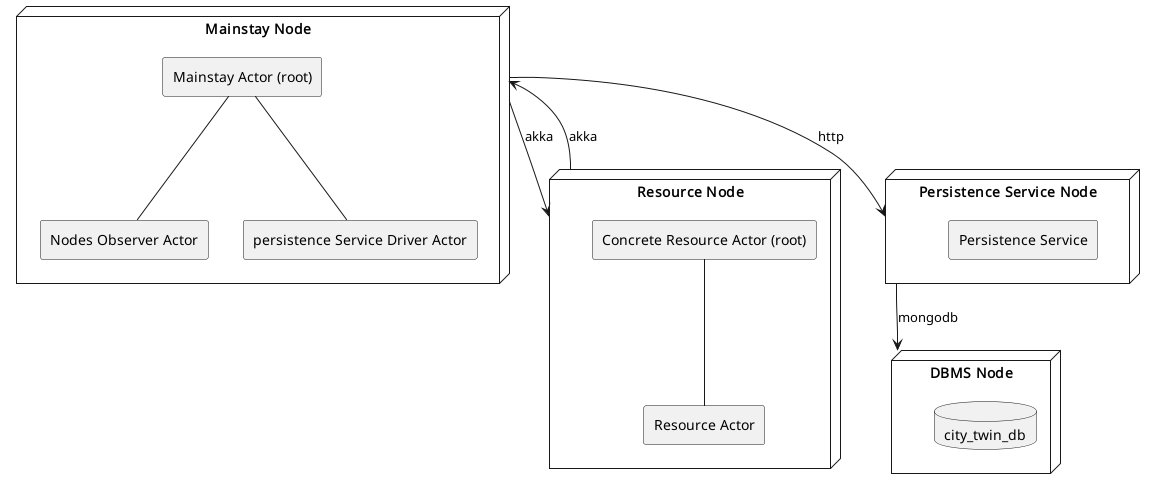
\includegraphics[width=\textwidth]{../assets/images/nodes-component-diagram.png}
\end{figure}

\begin{figure}[h]
    \caption{Diagramma di sequenza per l'aggiornamento dello stato di nodi del sistema.}
    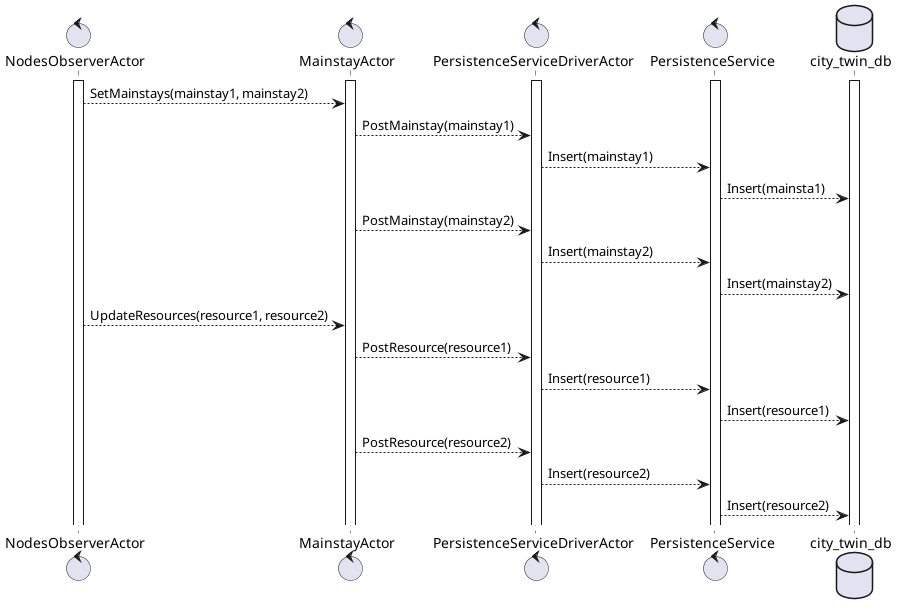
\includegraphics[width=\textwidth]{../assets/images/core-nodes-state-sequence-diagram.png}
\end{figure}

\begin{figure}[h]
    \caption{Diagramma di sequenza per lo scambio dello stato delle risorse.}
    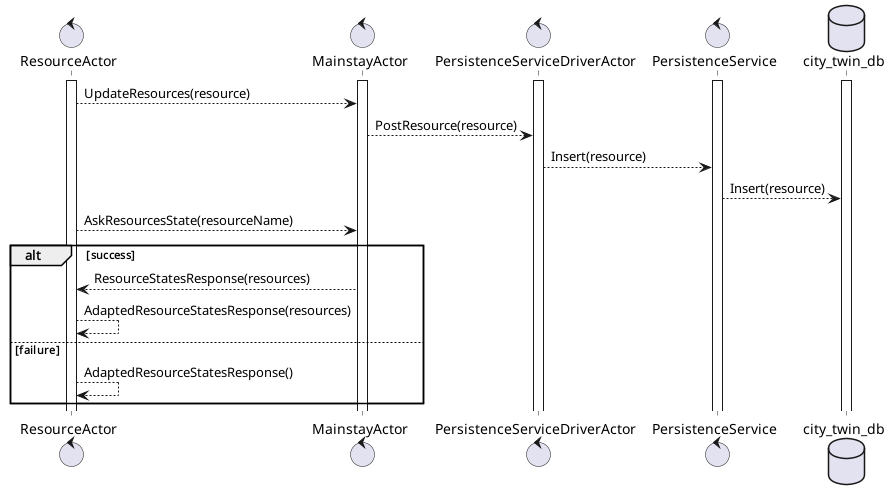
\includegraphics[width=\textwidth]{../assets/images/core-resource-state-exchange-sequence-diagram.png}
\end{figure}

\begin{figure}[h]
    \caption{Diagramma di sequenza per la sincronizzazione dei nodi Mainstay.}
    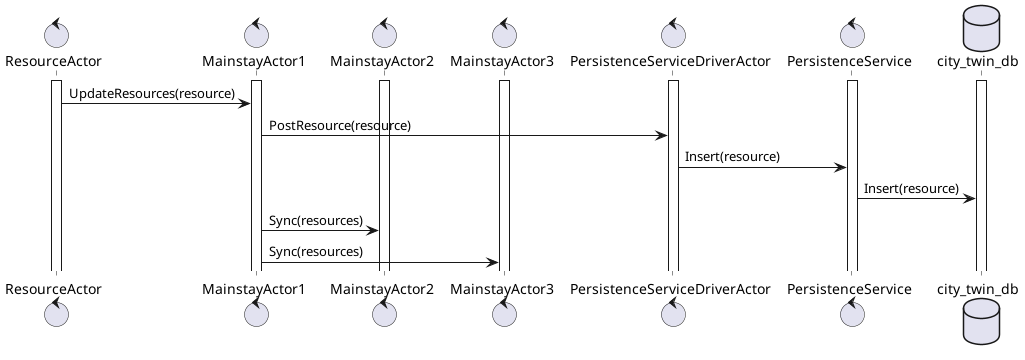
\includegraphics[width=\textwidth]{../assets/images/core-mainstays-sync-sequence-diagram.png}
\end{figure}

\begin{figure}[h]
    \caption{Diagramma di sequenza per l'aggiornamento del pannello di controllo.}
    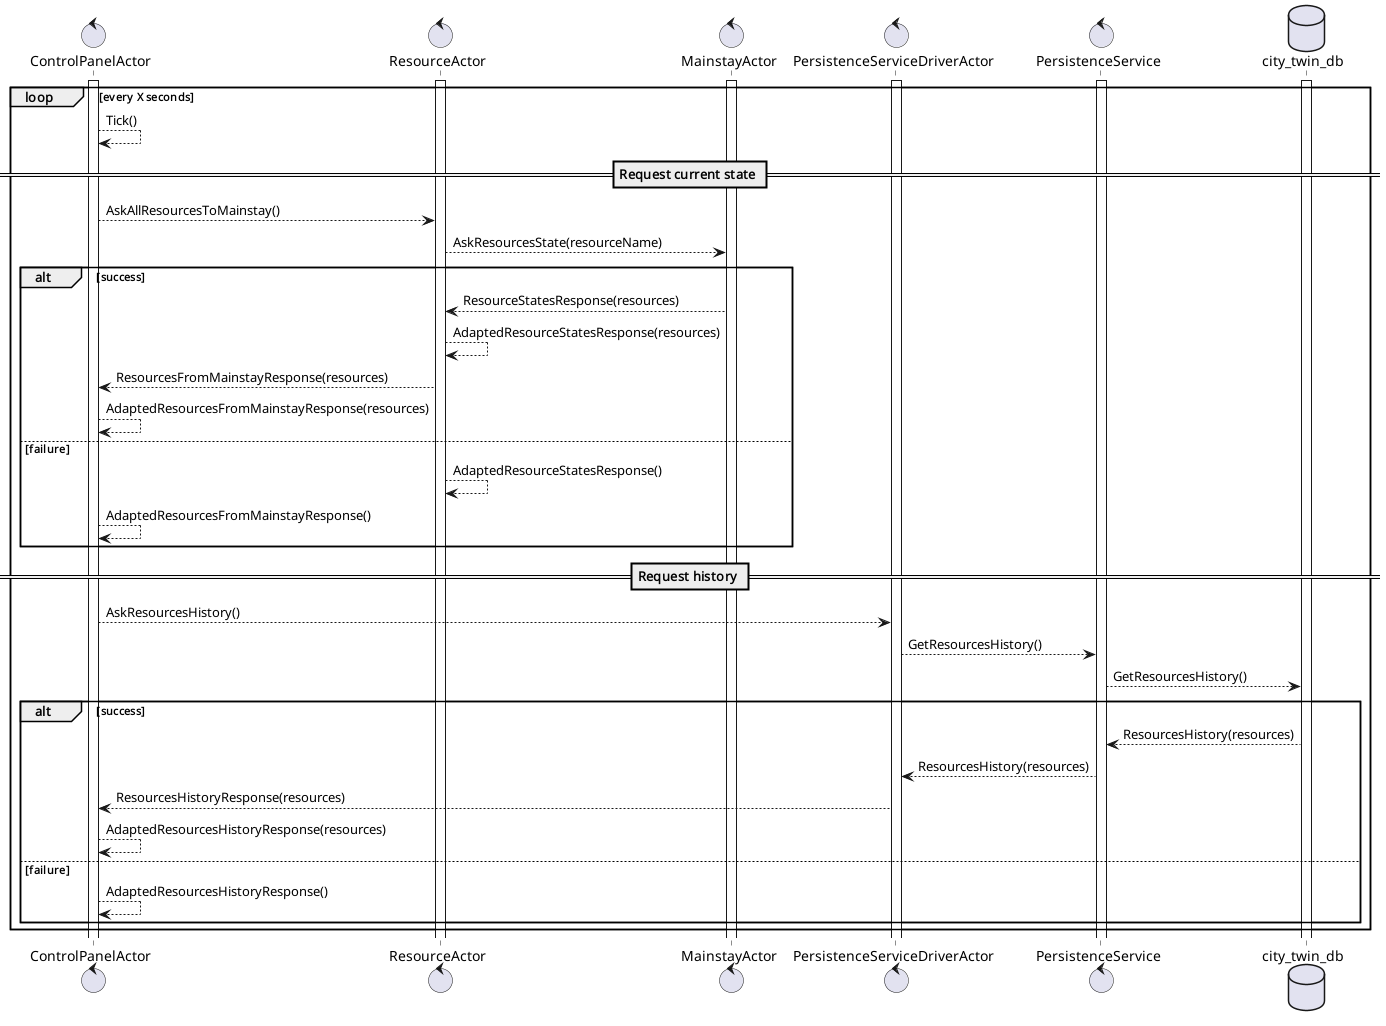
\includegraphics[width=\textwidth]{../assets/images/control-panel-sequence-diagram.png}
\end{figure}

\newpage

%----------------------------------------------------------------------------------------
%	IMPLEMENTAZIONE
%----------------------------------------------------------------------------------------

\section{Implementazione}\label{sec:implementazione}

\begin{figure}[h]
    \caption{Pannello di controllo: schermata della mappa della città.}
    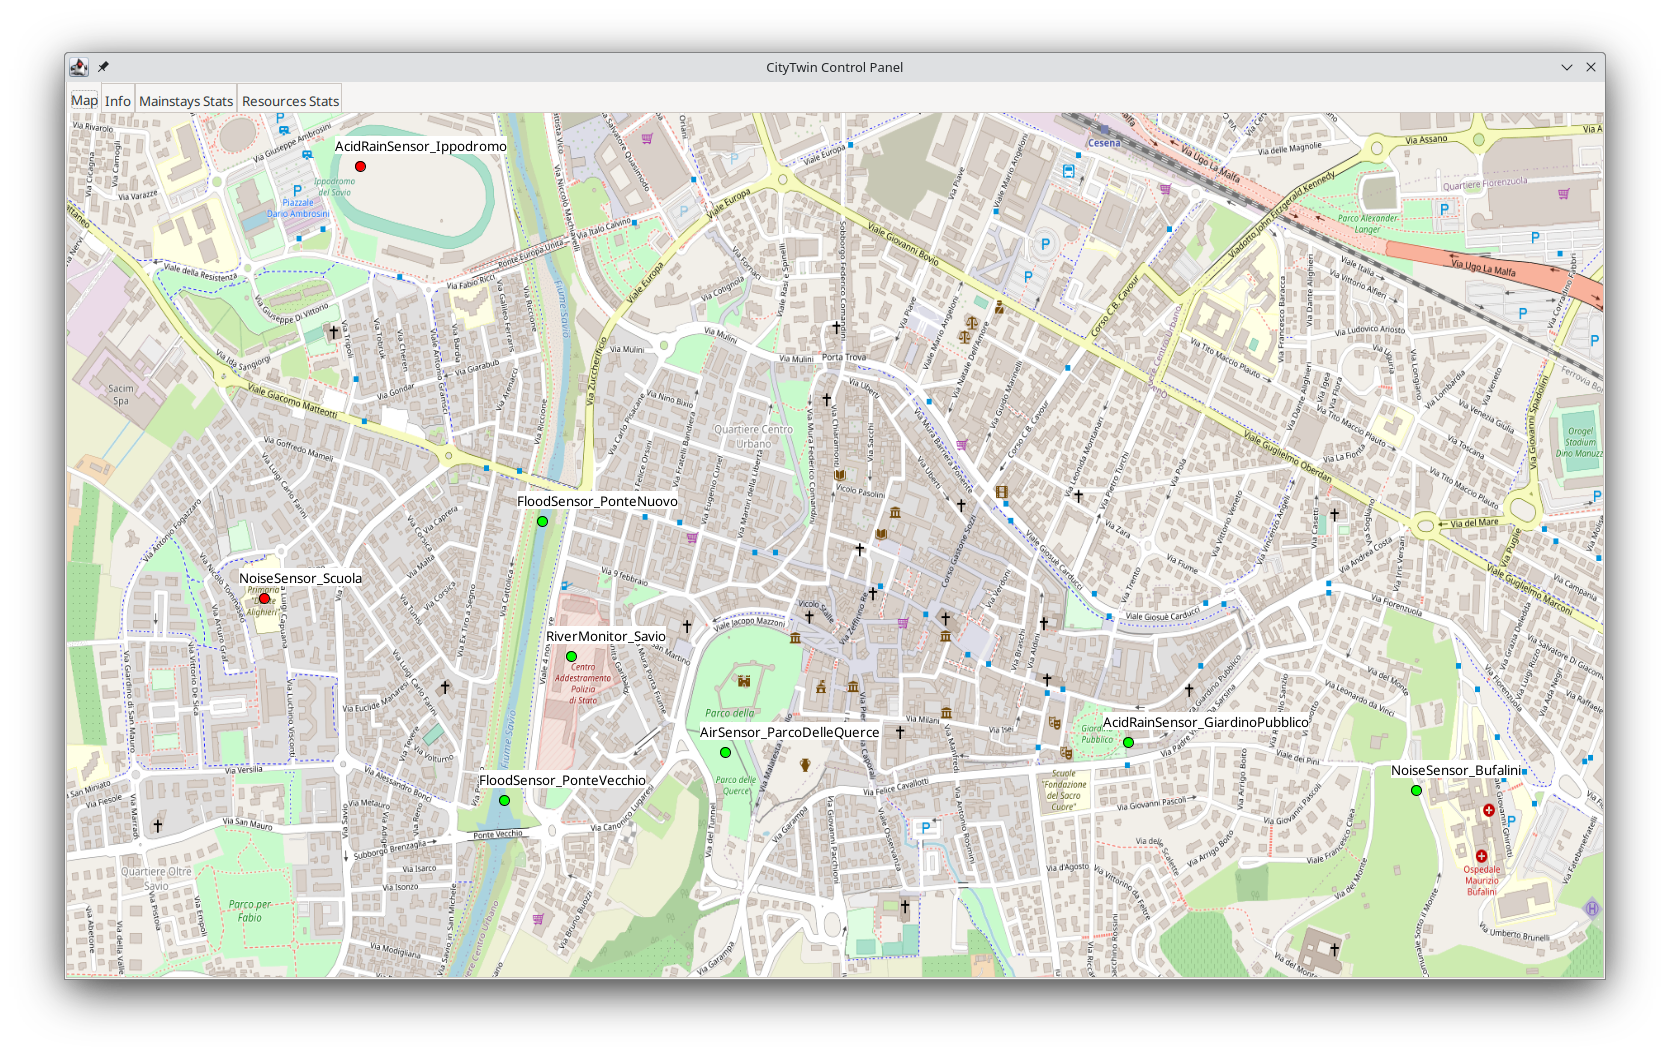
\includegraphics[width=\textwidth]{../assets/images/control-panel-map.png}
\end{figure}

\begin{figure}[h]
    \caption{Pannello di controllo: schermata delle informazioni sullo stato dei nodi \textit{Resource} e dei nodi \textit{Mainstay}.}
    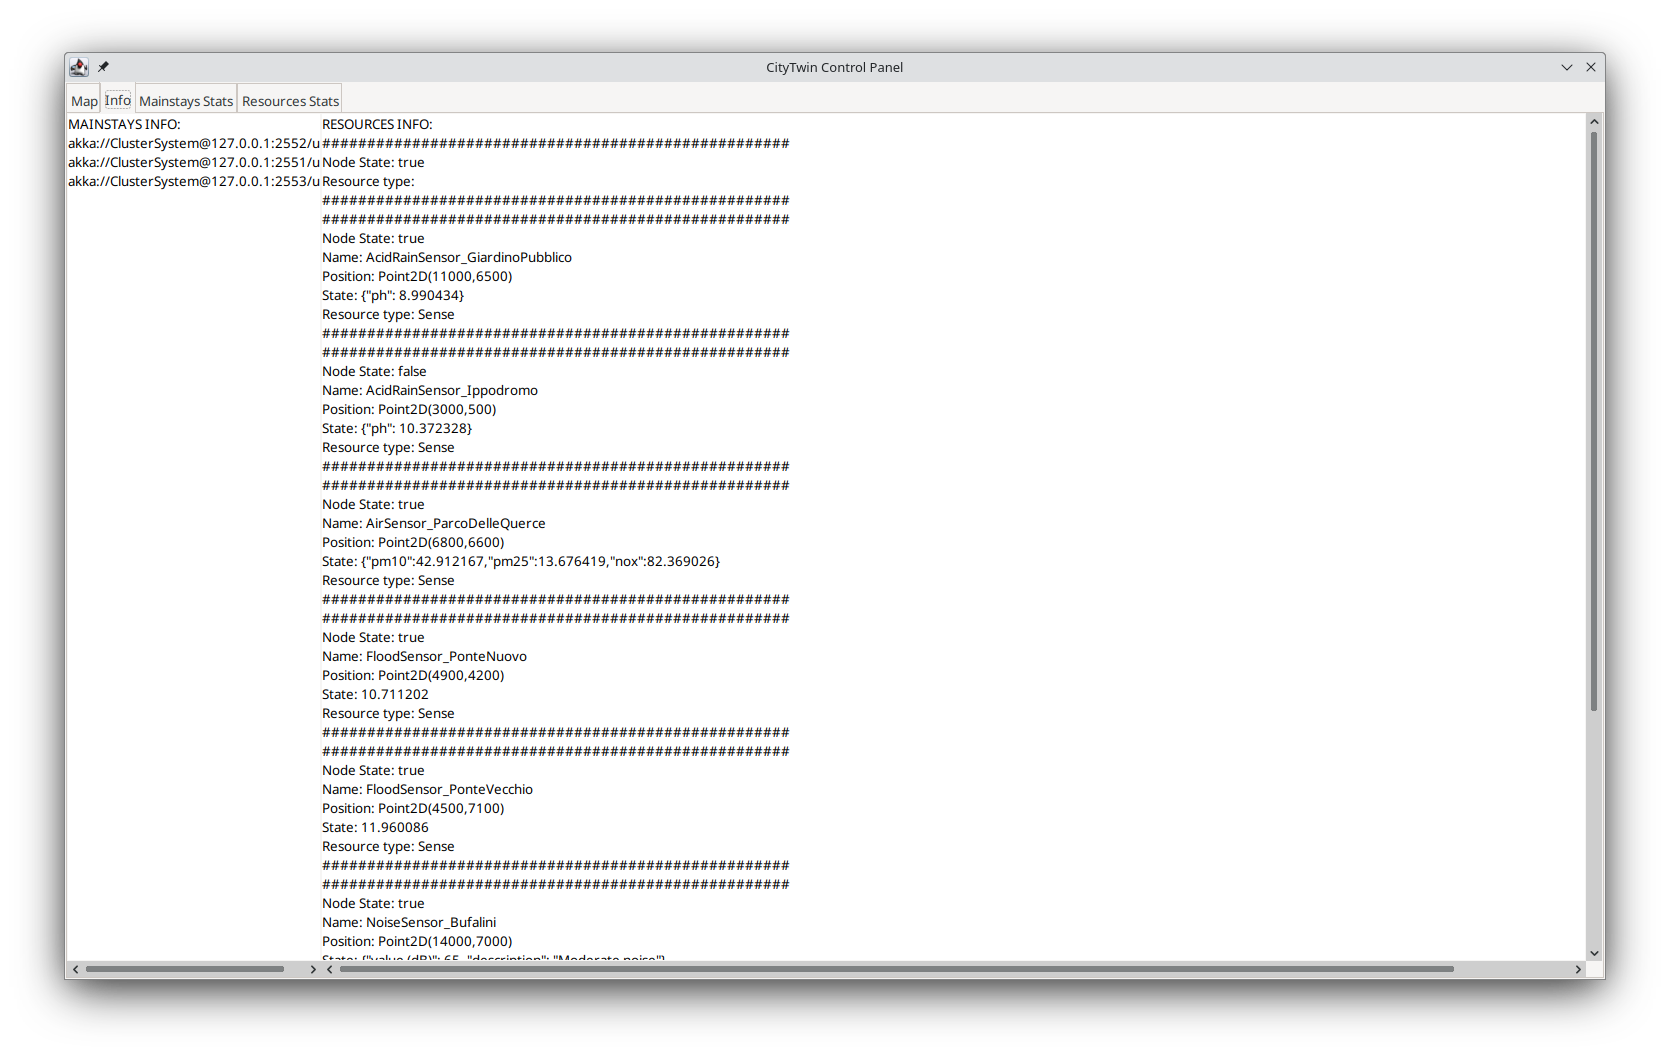
\includegraphics[width=\textwidth]{../assets/images/control-panel-info.png}
\end{figure}

\begin{figure}[h]
    \caption{Pannello di controllo: schermata delle statistiche dei nodi \textit{Resource}.}
    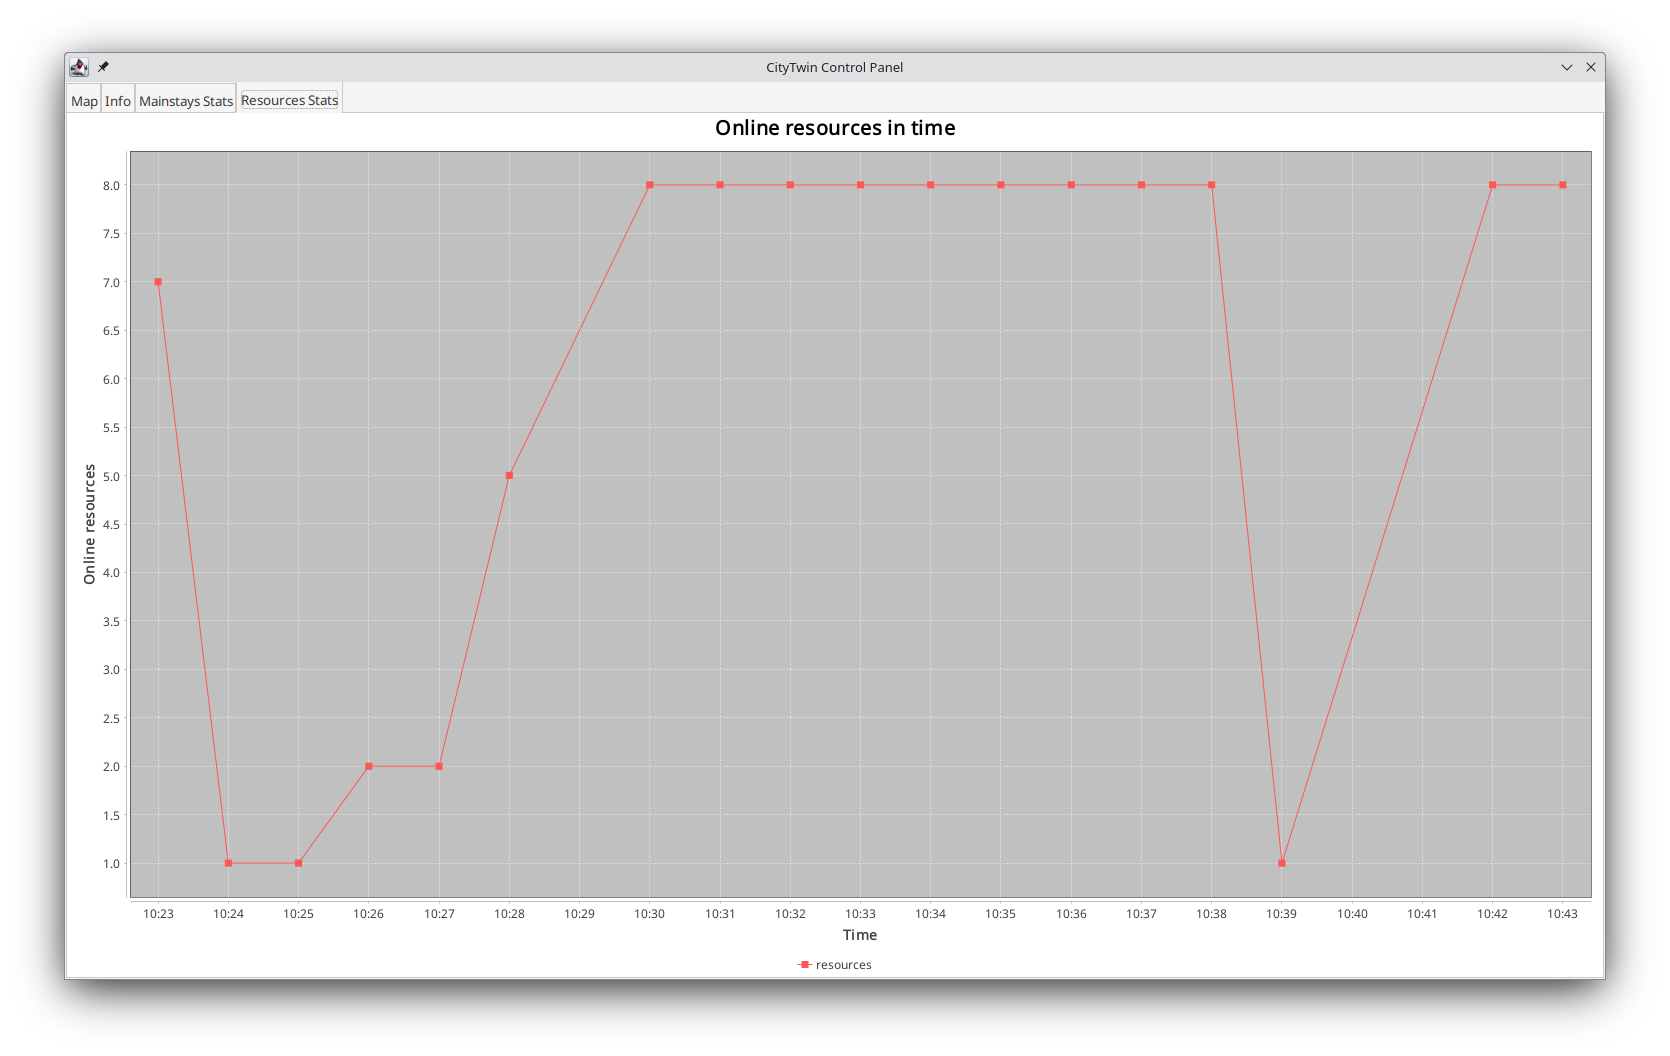
\includegraphics[width=\textwidth]{../assets/images/control-panel-resources-stats.png}
\end{figure}

\newpage


%----------------------------------------------------------------------------------------
%	TESTING E PERFORMANCE
%----------------------------------------------------------------------------------------

\section{Testing e performance}



\newpage


%----------------------------------------------------------------------------------------
%	ANALISI DI DEPLOYMENT SU LARGA SCALA
%----------------------------------------------------------------------------------------

\section{Analisi di deployment su larga scala}



\newpage


%----------------------------------------------------------------------------------------
%	PIANO DI LAVORO
%----------------------------------------------------------------------------------------

\section{Piano di lavoro}



\newpage


%----------------------------------------------------------------------------------------
%	CONCLUSIONI
%----------------------------------------------------------------------------------------

\section{Conclusioni}



\newpage


%----------------------------------------------------------------------------------------
%	APPENDICE
%----------------------------------------------------------------------------------------

\appendix
\addcontentsline{toc}{section}{Appendice}
\section*{Appendice}



\newpage


%----------------------------------------------------------------------------------------
%	RIFERIMENTI BIBLIOGRAFICI
%----------------------------------------------------------------------------------------
\addcontentsline{toc}{section}{Riferimenti bibliografici}
\begin{thebibliography}
    Elencare i riferimenti bibliografici citati nel testo.
\end{thebibliography}

%----------------------------------------------------------------------------------------

\end{document}